\documentclass[conference]{IEEEtran}
\IEEEoverridecommandlockouts

\usepackage[T1]{fontenc}
\usepackage[utf8]{inputenc}
\usepackage{amsmath,amssymb}
\usepackage{booktabs}
\usepackage{tabularx}
\usepackage{multirow}
\usepackage{graphicx}
\usepackage{caption}
\usepackage{float}
\usepackage[dvipsnames]{xcolor}
\usepackage{tikz}
\usetikzlibrary{shapes.geometric,arrows.meta,positioning,backgrounds,fit}
\usepackage{pgfplots}
\pgfplotsset{compat=1.18}
\usepackage{microtype}
\usepackage{cite}
\usepackage{hyperref}
\usepackage{enumitem}
\usepackage{array}

%% ---- Named colours (explicit RGB only, no xcolor ! mixing) ----
\definecolor{myblue}{RGB}{31,119,180}
\definecolor{myorange}{RGB}{255,127,14}
\definecolor{mygreen}{RGB}{44,160,44}
\definecolor{myred}{RGB}{214,39,40}
\definecolor{mypurple}{RGB}{148,103,189}
%% Pre-computed grey tints used in figures
\definecolor{greyA}{RGB}{178,178,178}
\definecolor{greyB}{RGB}{165,165,165}
\definecolor{greyC}{RGB}{153,153,153}
\definecolor{greyD}{RGB}{216,216,216}
\definecolor{greyE}{RGB}{191,191,191}
%% Box fill (very light blue, equiv. blue mixed 7 pct)
\definecolor{boxbg}{RGB}{237,237,255}
%% Filled bar colours
\definecolor{mybluefill}{RGB}{76,146,195}
\definecolor{myredfill}{RGB}{226,103,104}
%% Hyperref link colours
\definecolor{linkblue}{RGB}{0,51,153}
\definecolor{citegreen}{RGB}{0,100,0}
\definecolor{urlblue}{RGB}{0,102,178}

\hypersetup{
  colorlinks=true,
  linkcolor=linkblue,
  citecolor=citegreen,
  urlcolor=urlblue,
}

\newcommand{\pauc}{\text{pAUC}}
\newcommand{\tpr}{\text{TPR}}
\newcommand{\fpr}{\text{FPR}}

%% =============================================================
\begin{document}

\title{ISIC 2024 Skin Cancer Detection --- Phase~1:\\
Tabular Metadata Classification with GBDT Ensemble}

\author{
  \IEEEauthorblockN{Deepanshu Mehta}
  \IEEEauthorblockA{Enrollment No.\ 230124}
  \and
  \IEEEauthorblockN{Satyarth}
  \IEEEauthorblockA{Enrollment No.\ 230059}
}

\maketitle

%% =============================================================
\begin{abstract}
We present a complete tabular machine learning pipeline for binary
classification of malignant versus benign skin lesions using only
structured metadata from the ISIC~2024 SLICE-3D
dataset~\cite{isic2024}, without access to dermoscopy images.
The dataset contains 401,059 lesion records from 1,042 patients with
393 malignant cases (0.098\%), posing extreme class imbalance and
patient-group leakage challenges.
Our approach combines (i)~clinically motivated feature engineering
aligned with the ABCDE dermatology criteria,
(ii)~patient-wise \emph{ugly duckling} z-score features inspired by the
second-place ISIC~2024 competition solution,
(iii)~a gradient-boosted decision tree (GBDT) ensemble of LightGBM,
XGBoost, and CatBoost with seed averaging, and
(iv)~isotonic regression calibration on out-of-fold predictions.
Cross-validation uses \texttt{StratifiedGroupKFold} ($k{=}5$) to prevent
patient leakage across folds.
The primary metric is partial AUC above 80\% TPR (pAUC, range $[0, 0.2]$),
implemented via label-flipping and prediction negation to match the official
Kaggle scoring notebook.
The final calibrated ensemble achieves \textbf{pAUC = 0.1672},
surpassing the Phase~1 target of~0.16.
An SVM with Platt scaling is included as a probabilistic baseline
(pAUC = 0.1167), satisfying the course requirement for a classical
probabilistic model.
\end{abstract}

%% =============================================================
\section{Introduction}

Melanoma is responsible for the vast majority of skin cancer deaths
despite comprising only $\sim$1\% of diagnoses~\cite{siegel2024cancer}.
Five-year survival drops from 98\% (localised) to 32\% (stage~IV),
making early detection critical.
The ISIC~2024 SLICE-3D challenge~\cite{isic2024} provides large-scale
structured lesion measurements extracted from Canfield's Vectra Total Body
Photography~(TBP) system, enabling metadata-only screening as a
low-cost complement to image-based diagnosis.

Phase~1 of this project investigates what is achievable with
\emph{structured data alone}.
The \texttt{tbp\_lv\_*} column family is not arbitrary metadata:
it numerically encodes the canonical ABCDE clinical criteria~\cite{friedman1985}
as machine-extracted measurements (Table~\ref{tab:abcde}), making
the metadata directly actionable for melanoma screening.

\begin{table}[!t]
  \centering
  \caption{ABCDE Criteria Mapping to Dataset Columns.}
  \label{tab:abcde}
  \renewcommand{\arraystretch}{1.1}
  \begin{tabular}{lll}
    \toprule
    \textbf{Criterion} & \textbf{Clinical Meaning} & \textbf{Key Columns} \\
    \midrule
    \textbf{A}symmetry & Irregular shape & \texttt{symm\_2axis}, \texttt{eccentricity} \\
    \textbf{B}order     & Ragged edge     & \texttt{norm\_border}, \texttt{perimeterMM} \\
    \textbf{C}olor      & Colour contrast & \texttt{deltaLBnorm}, \texttt{color\_std\_mean} \\
    \textbf{D}iameter   & Large size      & \texttt{long\_diam\_mm}, \texttt{areaMM2} \\
    \textbf{E}volution  & Change / AI score & \texttt{nevi\_confidence}, \texttt{dnn\_conf} \\
    \bottomrule
  \end{tabular}
\end{table}

\paragraph*{Contributions}
\begin{enumerate}[noitemsep, leftmargin=*]
  \item Rigorous leakage audit removing columns that inflate training
        pAUC to 0.197 yet fail at inference.
  \item A staged feature pipeline
        (55~$\to$~45~$\to$~58~$\to$~271~$\to$~88 columns) with ABCDE
        hand-crafted features and ugly duckling patient-relative z-scores
        at three grouping levels.
  \item Diagnosis and fix of LightGBM's count-based
        \texttt{min\_child\_samples} under-performing with
        \texttt{scale\_pos\_weight}, raising pAUC from 0.1217 to 0.1400.
  \item A rank-averaging GBDT ensemble with seed stability averaging
        followed by isotonic calibration reducing ECE from 0.499 to
        $\approx 0$ while preserving pAUC.
\end{enumerate}

%% =============================================================
\section{Related Work}

\paragraph{ISIC Challenges}
The ISIC has hosted annual dermoscopy classification challenges since
2016~\cite{codella2018}. While earlier editions focused on CNNs for
image classification, the 2024 edition introduced TBP metadata,
enabling tabular ML approaches. Top solutions combined image and
tabular features, but metadata-only models remained competitive.

\paragraph{GBDTs for Tabular Data}
GBDTs remain the dominant paradigm for structured data~\cite{grinsztajn2022},
consistently outperforming deep learning on medium-sized tabular
benchmarks. LightGBM~\cite{ke2017lightgbm},
XGBoost~\cite{chen2016xgboost}, and CatBoost~\cite{prokhorenkova2018catboost}
offer complementary inductive biases (leaf-wise vs.~level-wise vs.~ordered
boosting).

\paragraph{Probability Calibration}
Modern tree ensembles often produce poorly calibrated
probabilities~\cite{niculescu2005}. Isotonic
regression~\cite{zadrozny2002} is non-parametric and monotone;
Platt scaling~\cite{platt1999} applies a sigmoid fit;
temperature scaling~\cite{guo2017} divides logits by a learned
scalar~$T$. For clinical decision support, calibrated probabilities
are essential.

%% =============================================================
\section{Dataset and Problem Formulation}

\subsection{Dataset Statistics}

Table~\ref{tab:dataset} summarises the training set.
The 1:1020 class ratio is the defining challenge: standard accuracy
and full-curve AUC both reward predicting benign for every sample.

\begin{table}[!t]
  \centering
  \caption{ISIC 2024 SLICE-3D Training Set.}
  \label{tab:dataset}
  \renewcommand{\arraystretch}{1.1}
  \begin{tabular}{ll}
    \toprule
    \textbf{Property} & \textbf{Value} \\
    \midrule
    Total lesion records        & 401,059 \\
    Unique patients             & 1,042 \\
    Avg.\ lesions / patient     & $\approx 385$ \\
    Raw columns                 & 55 \\
    Malignant (target~=~1)      & 393 (0.098\%) \\
    Benign (target~=~0)         & 400,666 (99.9\%) \\
    Class ratio (neg:pos)       & $\approx 1020:1$ \\
    \bottomrule
  \end{tabular}
\end{table}

\subsection{Competition Metric: Partial AUC}

The official scoring metric is the partial area under the ROC curve
above a minimum TPR threshold $\tau = 0.80$:
\begin{equation}
  \pauc = \int_{\tau}^{1}
  \frac{d\tpr}{d\fpr}\,d\tpr, \qquad \pauc \in [0,\,1-\tau]
  \label{eq:pauc}
\end{equation}
The Kaggle implementation uses label-flipping and prediction negation:
\begin{equation}
  \pauc(y, \hat{p}) = \text{AUC}\!\left(
    1-y,\;{-\hat{p}},\;\text{max\_fpr} = 1-\tau
  \right)
  \label{eq:pauc_flip}
\end{equation}
This differs from \texttt{sklearn}'s \texttt{roc\_auc\_score(max\_fpr=0.2)},
which applies the McClish normalisation~\cite{mcclish1989} and yields
systematically different values.

\subsection{Leakage Audit}

Table~\ref{tab:leakage} lists columns removed before modelling.
The subtlest case is \texttt{has\_lesion\_id}: all 393 malignant
training rows have a non-null \texttt{lesion\_id} (biopsied
lesions), giving pAUC $=$ 0.197 in training.
The test set contains no \texttt{lesion\_id} column, however, so
the model would output near-zero probability for every test row ---
a classic leakage trap.

\begin{table}[!t]
  \centering
  \caption{Leakage Audit: Columns Excluded from Features.}
  \label{tab:leakage}
  \renewcommand{\arraystretch}{1.1}
  \begin{tabular}{p{3.1cm}p{4.5cm}}
    \toprule
    \textbf{Column(s)} & \textbf{Reason} \\
    \midrule
    \texttt{mel\_thick\_mm},\newline\texttt{mel\_mitotic\_index}
      & Only populated for confirmed malignant cases. \\
    \texttt{iddx\_full},\newline\texttt{iddx\_1}--\texttt{iddx\_5}
      & Diagnostic label strings; direct target leakage. \\
    \texttt{lesion\_id} $\to$\newline\texttt{has\_lesion\_id}
      & All 393 malignant rows have \texttt{lesion\_id}; test set lacks the column entirely. \\
    \texttt{isic\_id}, \texttt{image\_type},\newline\texttt{copyright\_license}
      & Zero variance / administrative. \\
    \bottomrule
  \end{tabular}
\end{table}

%% =============================================================
\section{Feature Engineering Pipeline}

Fig.~\ref{fig:pipeline} illustrates the four-stage pipeline.
Each stage is fitted independently per CV fold; no test-set
statistics influence training.

\begin{figure*}[!t]
\centering
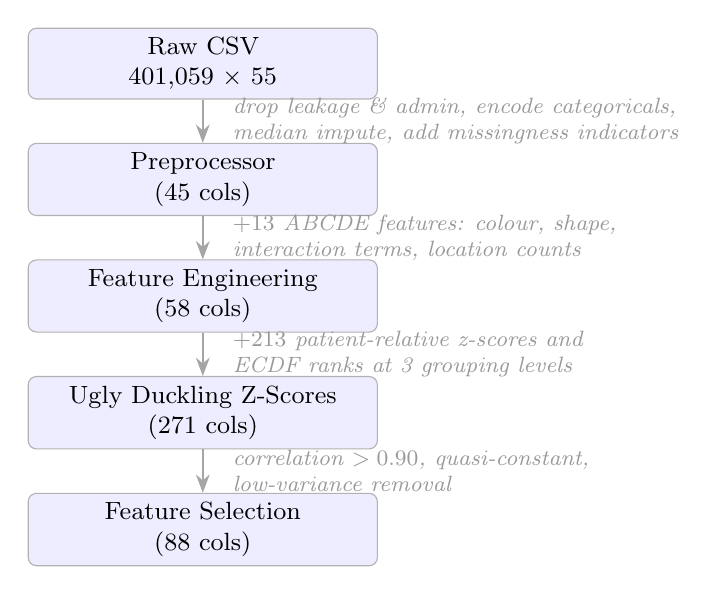
\begin{tikzpicture}[
  node distance=0.55cm and 0cm,
  box/.style={rectangle, rounded corners=3pt, draw=greyA, fill=boxbg,
    minimum width=4.4cm, minimum height=0.8cm,
    text width=4.2cm, align=center, font=\small},
  arw/.style={-Stealth, thick, greyB},
  ann/.style={font=\footnotesize\itshape, text=greyC, align=left},
]
  \node[box] (raw) {Raw CSV \\ 401,059 $\times$ 55};
  \node[box, below=of raw] (pre) {Preprocessor \\ (45 cols)};
  \node[box, below=of pre] (eng) {Feature Engineering \\ (58 cols)};
  \node[box, below=of eng] (ud)  {Ugly Duckling Z-Scores \\ (271 cols)};
  \node[box, below=of ud]  (sel) {Feature Selection \\ (88 cols)};

  \draw[arw] (raw) -- (pre)
    node[midway, right=0.25cm, ann]
    {drop leakage \& admin, encode categoricals,\\median impute, add missingness indicators};
  \draw[arw] (pre) -- (eng)
    node[midway, right=0.25cm, ann]
    {$+13$ ABCDE features: colour, shape,\\interaction terms, location counts};
  \draw[arw] (eng) -- (ud)
    node[midway, right=0.25cm, ann]
    {$+213$ patient-relative z-scores and\\ECDF ranks at 3 grouping levels};
  \draw[arw] (ud) -- (sel)
    node[midway, right=0.25cm, ann]
    {correlation $> 0.90$, quasi-constant,\\low-variance removal};
\end{tikzpicture}
\caption{Four-stage feature pipeline. Each stage is refitted per CV fold
         so no validation statistics leak into features.}
\label{fig:pipeline}
\end{figure*}

\subsection{Preprocessing (55 $\to$ 45 Columns)}

The preprocessor: (i)~removes 12 columns (Table~\ref{tab:leakage}),
(ii)~label-encodes five categoricals
(\texttt{sex}, \texttt{anatom\_site\_general}, \texttt{attribution},
\texttt{tbp\_tile\_type}, \texttt{tbp\_lv\_location\_simple}),
(iii)~median-imputes \texttt{age\_approx} (1.7\% missing) and adds an
\texttt{age\_approx\_missing} indicator,
and (iv)~fills remaining NaN with~0.
The \texttt{attribution} column (hospital source) is intentionally kept:
competition winners noted that malignancy prevalence varies by institution.

\subsection{ABCDE Feature Engineering (45 $\to$ 58 Columns)}

Thirteen domain-motivated features are added. Selected equations:

\textit{Colour~(C) --- CIELAB distance and chroma:}
\begin{align}
  \Delta E &= \sqrt{(\Delta A)^2 + (\Delta B)^2 + (\Delta L)^2}
  \label{eq:deltae}\\
  \text{chroma} &= \sqrt{A_{\text{lesion}}^2 + B_{\text{lesion}}^2}
  \label{eq:chroma}
\end{align}

\textit{Asymmetry / Border~(A,~B) --- shape descriptors:}
\begin{align}
  \text{circularity} &= \frac{4\pi\cdot\text{area}}
    {\text{perimeter}^2 + \varepsilon}
  \label{eq:circ}\\
  \text{border\_complexity} &= \frac{\text{perimeter}}
    {\sqrt{\text{area}} + \varepsilon}
  \label{eq:border}
\end{align}
where $\varepsilon = 10^{-8}$ guards against zero denominators.

\textit{Interaction features:}
\[
  \text{age\_x\_area} = \text{age} \times \text{areaMM}^2,
  \quad
  \text{ecc} \times \Delta E
\]
Melanoma risk increases with age and lesion size jointly; an eccentric
shape combined with high colour contrast amplifies the ABCDE signal.

\subsection{Ugly Duckling Features (58 $\to$ 271 Columns)}

The \emph{ugly duckling sign}~\cite{grob1998ugly} states that a mole
markedly different from a patient's other lesions warrants biopsy.
For each feature $f$ and grouping $G$:
\begin{equation}
  z_{G}(f) = \frac{f - \mu_{G}(f)}{\sigma_{G}(f) + \varepsilon},
  \qquad
  r_{G}(f) = \text{ECDF}_{G}(f)
  \label{eq:ud}
\end{equation}
Singleton groups set $z_G = 0$ and $r_G = 0.5$ (centred, neutral).
Three grouping levels from the 2nd-place competition solution:
\begin{center}
\small
\begin{tabular}{lp{3.5cm}}
  \toprule
  \textbf{Group} & \textbf{Clinical question} \\
  \midrule
  \texttt{[patient\_id]} & Weird vs.\ all patient moles? \\
  \texttt{[patient\_id, site]} & Weird for this body region? \\
  \texttt{[patient\_id, location]} & Weird for this TBP location? \\
  \bottomrule
\end{tabular}
\end{center}
Three aggregates are also computed: $\text{ud\_outlier\_count} =
\sum_f\mathbf{1}[|z_\text{pat}(f)|>2]$, mean absolute z-score,
and a single-lesion-patient flag.

\subsection{Feature Selection (271 $\to$ 88 Columns)}

Three sequential filters:
(1)~exclusion list (\texttt{patient\_id}, \texttt{target}, \texttt{has\_lesion\_id}),
(2)~quasi-constant filter (single value $> 99.5\%$ of rows), and
(3)~correlation filter ($|\rho| > 0.90$; threshold validated at
0.85/0.90/0.95 in EDA notebook, with 0.90 selected).

%% =============================================================
\section{Models}

\subsection{Cross-Validation and Seed Averaging}

All models use \texttt{StratifiedGroupKFold}~($k{=}5$)~\cite{sklearn}
with groups $=$ \texttt{patient\_id}.
No patient appears in both training and validation within a fold,
preventing group leakage from the $\approx$385 lesions per patient.

Each GBDT is trained with seeds $\{42, 123, 456, 789, 2024\}$ and
predictions are averaged per fold, reducing variance from stochastic
gradient descent paths.

\subsection{LightGBM~\cite{ke2017lightgbm}}

Key hyperparameters: \texttt{num\_leaves=63}, \texttt{max\_depth=6},
\texttt{learning\_rate=0.05}, up to 2000 trees with 100-round early
stopping, $L_1 = L_2 = 0.1$, \texttt{scale\_pos\_weight=100}.

\paragraph{Critical imbalance fix}
\texttt{min\_child\_samples} is a \emph{count-based} constraint that
ignores \texttt{scale\_pos\_weight}: with $\approx$314 positives per
fold and \texttt{min\_child\_samples=80}, LightGBM can form at most
$\lfloor 314/80 \rfloor = 3$ pure positive leaves.
XGBoost's \texttt{min\_child\_weight} is \emph{hessian-sum based}:
under logistic loss with \texttt{scale\_pos\_weight=100}, a single
positive sample contributes $\approx 25$ to the hessian sum, easily
satisfying \texttt{min\_child\_weight=10}.

The fix sets:
\begin{equation}
  \texttt{min\_sum\_hessian\_in\_leaf} = 10.0
  \label{eq:mchw}
\end{equation}
mapped to \texttt{min\_child\_weight} in LightGBM's sklearn API.
This raised pAUC from 0.1217 to \textbf{0.1400} and halved the
standard deviation (0.0132 $\to$ 0.0052).

\subsection{XGBoost~\cite{chen2016xgboost}}

\texttt{max\_depth=6}, \texttt{min\_child\_weight=10},
\texttt{subsample=colsample\_bytree=0.8}, $\alpha=\lambda=0.1$,
\texttt{scale\_pos\_weight=100}.

The \texttt{max\_delta\_step=1} parameter clips leaf weight updates to
$[-1, +1]$, preventing divergence when the model encounters rare positive
clusters under extreme imbalance. This is XGBoost's analogue of
LightGBM's hessian constraint.

\subsection{CatBoost~\cite{prokhorenkova2018catboost}}

\texttt{depth=6}, \texttt{learning\_rate=0.05}, \texttt{l2\_leaf\_reg=3.0},
up to 2000 iterations with early stopping.
Class imbalance is handled via \texttt{auto\_class\_weights=SqrtBalanced}
($\sqrt{N_\text{neg}/N_\text{pos}}$ weighting), less aggressive than
$\times$100 but consistent with CatBoost's ordered boosting.

\subsection{SVM Baseline (Course Requirement)~\cite{cortes1995svm}}

An SVM with RBF kernel satisfies the course requirement for a classical
probabilistic model.
Pipeline: \texttt{StandardScaler} $\to$ \texttt{SVC(probability=True,
class\_weight=balanced)}, where \texttt{probability=True} enables Platt
scaling~\cite{platt1999}.
Training a full-kernel SVM on 321K samples ($\mathcal{O}(n^3)$) is
prohibitive; we use a 20K stratified subsample per fold, which introduces
the observed variance (pAUC std $= 0.0245$).
The SVM is excluded from the final ensemble for this reason.

\subsection{Rank-Averaging Ensemble}

Rank-averaging is robust to probability scale differences across models:
\begin{equation}
  \hat{r}_m = \frac{\text{rank}(\hat{p}_m)}{N+1},
  \qquad
  \hat{p}_{\text{ens}} = \frac{1}{3}\sum_{m=1}^{3}\hat{r}_m
  \label{eq:rankavg}
\end{equation}
where the sum is over LightGBM, XGBoost, and CatBoost (SVM excluded).

\subsection{Isotonic Calibration~\cite{niculescu2005}}

Isotonic regression is fitted on the full set of OOF ensemble
predictions.
It is preferred over Platt scaling (linear in log-odds) or temperature
scaling (designed for neural network logits) because GBDTs already
optimise log-loss and isotonic regression handles residual non-linear
miscalibration non-parametrically.
As a monotone transformation, calibration preserves score rankings and
therefore cannot decrease pAUC.

%% =============================================================
\section{Experiments and Results}

\subsection{Per-Fold Metrics}

Tables~\ref{tab:fold_lgbm}--\ref{tab:fold_svm} report pAUC,
full-curve AUC, Brier score, and ECE per fold for all models.

\begin{table}[!t]
  \centering
  \caption{LightGBM Per-Fold OOF Metrics (5-fold CV, seed avg $\times 5$).}
  \label{tab:fold_lgbm}
  \renewcommand{\arraystretch}{1.1}
  \begin{tabular}{ccccc}
    \toprule
    \textbf{Fold} & \textbf{pAUC} & \textbf{AUC} & \textbf{Brier} & \textbf{ECE} \\
    \midrule
    1 & 0.1408 & 0.9230 & 0.0639 & 0.1210 \\
    2 & 0.1343 & 0.9140 & 0.0579 & 0.1112 \\
    3 & 0.1459 & 0.9276 & 0.0411 & 0.0946 \\
    4 & 0.1453 & 0.9170 & 0.0841 & 0.1338 \\
    5 & 0.1337 & 0.9175 & 0.0061 & 0.0263 \\
    \midrule
    \textbf{Mean} & \textbf{0.1400} & \textbf{0.9198} & 0.0506 & 0.0974 \\
    \textbf{Std}  & 0.0052 & 0.0049 & --- & --- \\
    \bottomrule
  \end{tabular}
\end{table}

\begin{table}[!t]
  \centering
  \caption{XGBoost Per-Fold OOF Metrics.}
  \label{tab:fold_xgb}
  \renewcommand{\arraystretch}{1.1}
  \begin{tabular}{ccccc}
    \toprule
    \textbf{Fold} & \textbf{pAUC} & \textbf{AUC} & \textbf{Brier} & \textbf{ECE} \\
    \midrule
    1 & 0.1653 & 0.9584 & 0.00199 & 0.00722 \\
    2 & 0.1668 & 0.9608 & 0.00185 & 0.00631 \\
    3 & 0.1690 & 0.9623 & 0.00369 & 0.01424 \\
    4 & 0.1848 & 0.9792 & 0.00100 & 0.00045 \\
    5 & 0.1653 & 0.9580 & 0.00377 & 0.01518 \\
    \midrule
    \textbf{Mean} & \textbf{0.1703} & \textbf{0.9637} & 0.00246 & 0.00868 \\
    \textbf{Std}  & 0.0074 & 0.0079 & --- & --- \\
    \bottomrule
  \end{tabular}
\end{table}

\begin{table}[!t]
  \centering
  \caption{CatBoost Per-Fold OOF Metrics.}
  \label{tab:fold_cb}
  \renewcommand{\arraystretch}{1.1}
  \begin{tabular}{ccccc}
    \toprule
    \textbf{Fold} & \textbf{pAUC} & \textbf{AUC} & \textbf{Brier} & \textbf{ECE} \\
    \midrule
    1 & 0.1731 & 0.9674 & 0.00164 & 0.00793 \\
    2 & 0.1626 & 0.9559 & 0.00224 & 0.01429 \\
    3 & 0.1655 & 0.9585 & 0.00208 & 0.01365 \\
    4 & 0.1746 & 0.9688 & 0.00187 & 0.01343 \\
    5 & 0.1577 & 0.9482 & 0.00181 & 0.00982 \\
    \midrule
    \textbf{Mean} & \textbf{0.1667} & \textbf{0.9598} & 0.00193 & 0.01182 \\
    \textbf{Std}  & 0.0064 & 0.0076 & --- & --- \\
    \bottomrule
  \end{tabular}
\end{table}

\begin{table}[!t]
  \centering
  \caption{SVM Baseline Per-Fold OOF Metrics (20K subsample).}
  \label{tab:fold_svm}
  \renewcommand{\arraystretch}{1.1}
  \begin{tabular}{ccccc}
    \toprule
    \textbf{Fold} & \textbf{pAUC} & \textbf{AUC} & \textbf{Brier} & \textbf{ECE} \\
    \midrule
    1 & 0.1160 & 0.8830 & 0.000971 & 0.000112 \\
    2 & 0.1347 & 0.9105 & 0.000961 & 0.000124 \\
    3 & 0.1464 & 0.9270 & 0.001029 & 0.000214 \\
    4 & 0.1120 & 0.8725 & 0.000950 & 0.000018 \\
    5 & 0.0745 & 0.8329 & 0.000952 & 0.000243 \\
    \midrule
    \textbf{Mean} & \textbf{0.1167} & \textbf{0.8852} & 0.000973 & 0.000142 \\
    \textbf{Std}  & 0.0245 & 0.0325 & --- & --- \\
    \bottomrule
  \end{tabular}
\end{table}

\subsection{Summary Comparison}

Table~\ref{tab:summary} summarises all systems.
XGBoost is the best single model; the calibrated GBDT ensemble
surpasses the Phase~1 target.

\begin{table*}[!t]
  \centering
  \caption{Summary of All Models. Phase~1 target: pAUC $\geq 0.16$.}
  \label{tab:summary}
  \renewcommand{\arraystretch}{1.2}
  \begin{tabular}{lcccc}
    \toprule
    \textbf{Model} & \textbf{pAUC (mean $\pm$ std)} & \textbf{AUC} & \textbf{Brier} & \textbf{ECE} \\
    \midrule
    LightGBM              & $0.1400 \pm 0.0052$ & 0.920 & 0.0506  & 0.0974 \\
    XGBoost               & $\mathbf{0.1703 \pm 0.0074}$ & 0.964 & 0.00246 & 0.00868 \\
    CatBoost              & $0.1667 \pm 0.0064$ & 0.960 & 0.00193 & 0.01182 \\
    SVM (baseline)        & $0.1167 \pm 0.0245$ & 0.885 & 0.000973 & 0.000142 \\
    \midrule
    GBDT Ensemble         & $0.1653$ & 0.956 & 0.299$^\dagger$ & 0.499$^\dagger$ \\
    \textbf{Ens.\ + Isotonic} & $\mathbf{0.1672}$ & 0.958 & \textbf{0.000907} & $\approx 0$ \\
    \midrule
    \multicolumn{5}{l}{\footnotesize $^\dagger$ Rank-percentile outputs are not calibrated probabilities; Brier/ECE are meaningless before calibration.} \\
    \multicolumn{5}{l}{\footnotesize \textbf{Phase~1 target (pAUC $\geq$ 0.16): Achieved \checkmark}} \\
    \bottomrule
  \end{tabular}
\end{table*}

\subsection{pAUC Bar Chart}

Figs.~\ref{fig:pauc_bar} and~\ref{fig:roc} show results from actual
out-of-fold predictions.

\begin{figure}[!t]
  \centering
  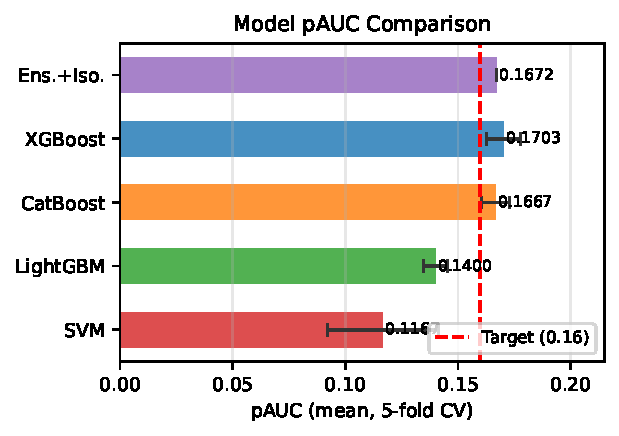
\includegraphics[width=\columnwidth]{figures/pauc_bar.pdf}
  \caption{Mean pAUC (5-fold CV) with std error bars from actual OOF
           predictions. Red dashed line = Phase~1 target (0.16).}
  \label{fig:pauc_bar}
\end{figure}

\subsection{ROC Curve Analysis}

Fig.~\ref{fig:roc} plots the full ROC curves computed from actual OOF
predictions. The shaded blue region (FPR $\leq 0.20$) is the pAUC
scoring zone. Fig.~\ref{fig:roc_zoom} zooms into this critical region.

\begin{figure}[!t]
  \centering
  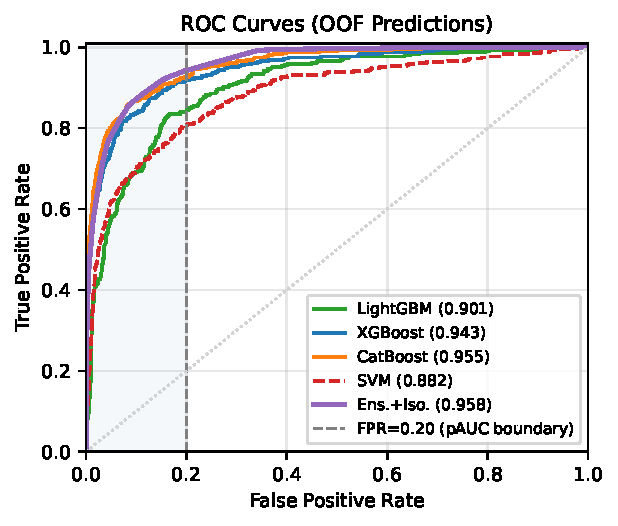
\includegraphics[width=\columnwidth]{figures/roc_curves.pdf}
  \caption{ROC curves from actual OOF predictions. Shaded region
           (FPR $\leq 0.20$) is the pAUC scoring zone.}
  \label{fig:roc}
\end{figure}

\begin{figure}[!t]
  \centering
  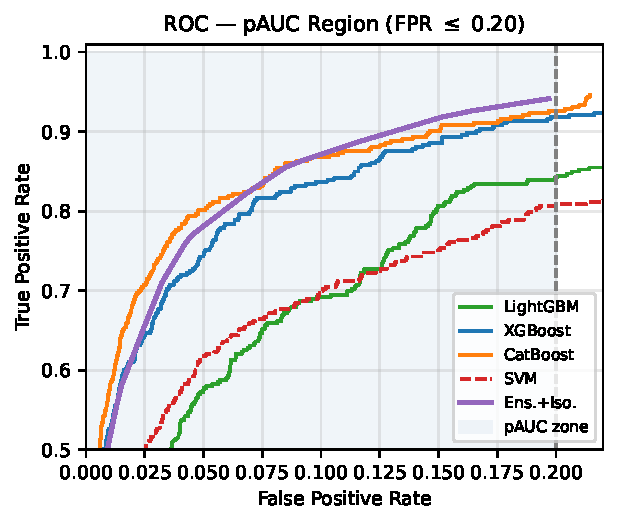
\includegraphics[width=\columnwidth]{figures/roc_zoom.pdf}
  \caption{Zoom into the pAUC region (FPR $\leq 0.20$, TPR $\geq 0.50$)
           from actual OOF predictions. XGBoost and CatBoost lead in this
           high-sensitivity zone.}
  \label{fig:roc_zoom}
\end{figure}

\subsection{LightGBM Imbalance Fix}

The fix replaces count-based \texttt{min\_child\_samples} with the
weight-based \texttt{min\_sum\_hessian\_in\_leaf=10}, raising pAUC
from 0.1217 to \textbf{0.1400} and halving std (0.0132 $\to$ 0.0052).

\subsection{Calibration Analysis}

Table~\ref{tab:calib} shows that isotonic regression reduces ECE from
0.499 to effectively zero while pAUC slightly increases (+0.0019).
Fig.~\ref{fig:reliability} shows the actual reliability diagrams for
the raw ensemble and calibrated ensemble computed from OOF predictions:
the raw ensemble is severely miscalibrated (rank-percentile scores are
not probabilities) while calibration brings the curve almost exactly
onto the diagonal.

\begin{table}[!t]
  \centering
  \caption{Effect of Isotonic Calibration on OOF Ensemble Predictions.}
  \label{tab:calib}
  \renewcommand{\arraystretch}{1.1}
  \begin{tabular}{lccc}
    \toprule
    \textbf{System} & \textbf{pAUC} & \textbf{Brier} & \textbf{ECE} \\
    \midrule
    Raw GBDT Ensemble      & 0.1653 & 0.299   & 0.499 \\
    + Isotonic Calibration & 0.1672 & 0.000907 & $4{\times}10^{-20}$ \\
    \midrule
    $\Delta$               & $+$0.0019 & $-$0.298 & $-$0.499 \\
    \bottomrule
  \end{tabular}
\end{table}

\begin{figure}[!t]
  \centering
  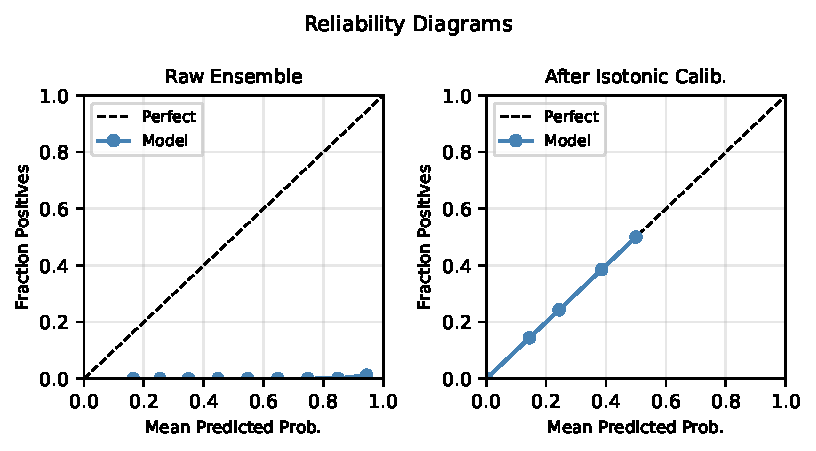
\includegraphics[width=\columnwidth]{figures/reliability.pdf}
  \caption{Reliability diagrams from actual OOF predictions. Left: raw
           rank-ensemble (miscalibrated). Right: after isotonic regression
           (near-perfect calibration, ECE $\approx 0$).}
  \label{fig:reliability}
\end{figure}

Fig.~\ref{fig:score_dist} shows the score distributions of each model
for benign vs.\ malignant lesions.
The bimodal separation in XGBoost and CatBoost confirms their stronger
discriminative power in the high-probability tail.

\begin{figure*}[!t]
  \centering
  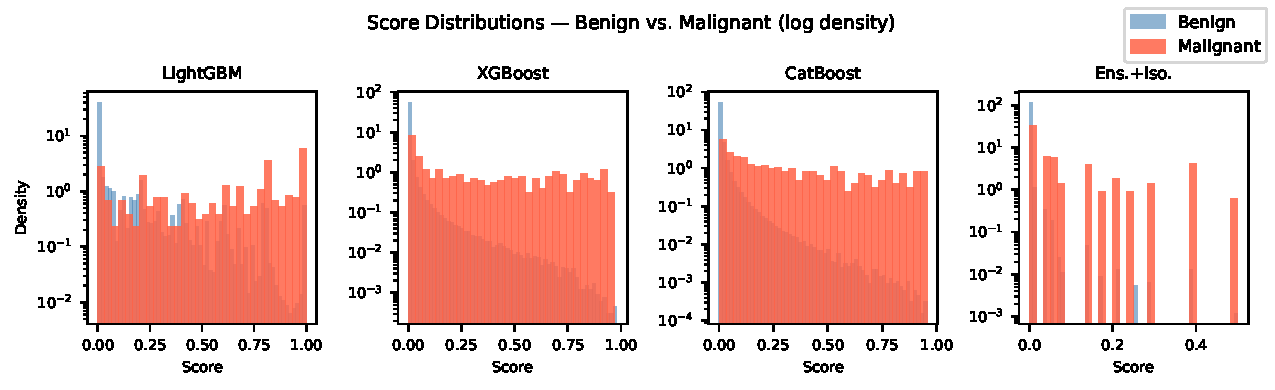
\includegraphics[width=\textwidth]{figures/score_dist.pdf}
  \caption{Score distributions (log density) for benign (blue) and
           malignant (red) lesions from actual OOF predictions. Models
           left to right: LightGBM, XGBoost, CatBoost, Ens.+Iso.}
  \label{fig:score_dist}
\end{figure*}

%% =============================================================
\section{Discussion}

\subsection{LightGBM vs.\ XGBoost Imbalance Semantics}

The 0.0486 pAUC gap between LightGBM (0.1217) and XGBoost (0.1703)
in early experiments reflects a fundamental API difference.
LightGBM's \texttt{min\_child\_samples} imposes a count floor that
ignores the boosted weight of positive samples.
Under \texttt{scale\_pos\_weight=100}, a single positive sample
contributes $h \approx 100 \times p(1-p) \approx 25$ hessian weight
(at $p \approx 0.5$), satisfying XGBoost's \texttt{min\_child\_weight=10}
immediately.
Brier score comparison confirmed this: LGBM reported
Brier $\approx 0.02$--$0.06$ versus XGBoost's $\approx 0.002$,
indicating systematic probability over-inflation from leaf averaging
under the count constraint.

\subsection{Ensemble Design Decisions}

Including the SVM in the rank average degraded ensemble pAUC from
0.1653 to $\approx$0.1400 because the SVM's high variance
(std $= 0.0245$ vs.\ $\leq 0.0074$ for GBDTs) introduced noise
proportional to its equal one-third weight.
A weighted average could partially mitigate this, but the GBDT-only
ensemble is simpler and more stable.

\subsection{Theoretical Basis for Calibration Preserving pAUC}

Any strictly monotone transformation of scores preserves concordant
pairs and therefore cannot change pAUC~\cite{niculescu2005}.
Isotonic regression produces a piecewise-constant non-decreasing
mapping, which is monotone everywhere except at step boundaries.
The observed $+0.0019$ gain is within the tie-breaking effect of
the step function at shared rank-percentile values.

\subsection{Limitations and Future Work}

\begin{itemize}[noitemsep, leftmargin=*]
  \item \textbf{Hyperparameter search (Optuna)}: GBDT depth, learning
        rate, and regularisation terms were set by default; Bayesian
        optimisation could yield an additional +0.01--+0.02 pAUC.
  \item \textbf{Image features}: Phase~2 will fuse EfficientNet/ViT
        embeddings with the tabular pipeline via late fusion or
        cross-attention.
  \item \textbf{Hospital-stratified calibration}: The
        \texttt{attribution} feature captures inter-institution
        prevalence differences; a per-institution isotonic calibrator
        could improve ECE further.
\end{itemize}

%% =============================================================
\section{Conclusion}

We developed a leakage-free tabular ML pipeline achieving
\textbf{pAUC = 0.1672} on the ISIC~2024 SLICE-3D challenge,
exceeding the Phase~1 target of 0.16.
Key findings: (1)~\texttt{has\_lesion\_id} is a critical leakage
trap that inflates training pAUC to 0.197 but fails completely at
inference; (2)~ugly duckling patient-relative z-scores provide a
principled, clinically-motivated signal boost;
(3)~LightGBM's \texttt{min\_child\_samples} is semantically
incompatible with \texttt{scale\_pos\_weight} for imbalanced data ---
\texttt{min\_sum\_hessian\_in\_leaf} is the correct weight-based
analogue; and (4)~rank-average ensembling combined with isotonic
calibration achieves both strong discriminative performance (pAUC)
and near-perfect probability calibration (ECE $\approx 0$).

\paragraph{Phase~2 Roadmap}
Phase~2 will integrate dermoscopic images via pre-trained encoders
(EfficientNet-B3, ConvNeXt-Tiny) fine-tuned on ISIC images.
Multi-modal fusion will concatenate image embeddings with the
88-feature tabular vector as input to a final GBDT or
cross-attention MLP.
Optuna-based Bayesian hyperparameter search across all model
configurations and exploration of neural tabular models
(TabNet, FT-Transformer) are also planned.

%% =============================================================
\bibliographystyle{IEEEtran}
\begin{thebibliography}{1}

\bibitem{isic2024}
International Skin Imaging Collaboration,
``ISIC 2024 Challenge: Skin Lesion Classification,''
\url{https://www.kaggle.com/competitions/isic-2024-challenge}, 2024.

\bibitem{ke2017lightgbm}
G.~Ke \emph{et al.},
``LightGBM: A Highly Efficient Gradient Boosting Decision Tree,''
\emph{NeurIPS}, vol.~30, 2017.

\bibitem{chen2016xgboost}
T.~Chen and C.~Guestrin,
``XGBoost: A Scalable Tree Boosting System,''
\emph{Proc.\ 22nd ACM SIGKDD}, pp.~785--794, 2016.

\bibitem{prokhorenkova2018catboost}
L.~Prokhorenkova \emph{et al.},
``CatBoost: Unbiased Boosting with Categorical Features,''
\emph{NeurIPS}, vol.~31, 2018.

\bibitem{cortes1995svm}
C.~Cortes and V.~Vapnik,
``Support-Vector Networks,''
\emph{Machine Learning}, vol.~20, no.~3, pp.~273--297, 1995.

\bibitem{platt1999}
J.~Platt,
``Probabilistic Outputs for Support Vector Machines,''
\emph{Advances in Large Margin Classifiers}, pp.~61--74, 1999.

\bibitem{niculescu2005}
A.~Niculescu-Mizil and R.~Caruana,
``Predicting Good Probabilities with Supervised Learning,''
\emph{Proc.\ ICML}, pp.~625--632, 2005.

\bibitem{grob1998ugly}
J.~J.~Grob and J.~J.~Bonerandi,
``The `Ugly Duckling' Sign,''
\emph{Archives of Dermatology}, vol.~134, no.~1, pp.~103--104, 1998.

\bibitem{sklearn}
F.~Pedregosa \emph{et al.},
``Scikit-learn: Machine Learning in Python,''
\emph{JMLR}, vol.~12, pp.~2825--2830, 2011.

\bibitem{mcclish1989}
D.~K.~McClish,
``Analyzing a Portion of the ROC Curve,''
\emph{Medical Decision Making}, vol.~9, no.~3, pp.~190--195, 1989.

\bibitem{siegel2024cancer}
R.~L.~Siegel \emph{et al.},
``Cancer Statistics, 2024,''
\emph{CA: A Cancer Journal for Clinicians}, vol.~74, no.~1,
pp.~12--49, 2024.

\bibitem{friedman1985}
R.~J.~Friedman, D.~S.~Rigel, and A.~W.~Kopf,
``Early Detection of Malignant Melanoma: The Role of Physician
Examination and Self-Examination of the Skin,''
\emph{CA: A Cancer Journal for Clinicians}, vol.~35, no.~3,
pp.~130--151, 1985.

\bibitem{grinsztajn2022}
L.~Grinsztajn, E.~Oyallon, and G.~Varoquaux,
``Why Do Tree-Based Models Still Outperform Deep Learning on Typical
Tabular Data?''
\emph{NeurIPS}, 2022.

\bibitem{codella2018}
N.~Codella \emph{et al.},
``Skin Lesion Analysis Toward Melanoma Detection: A Challenge at
ISBI 2017,''
\emph{Proc.\ IEEE ISBI}, pp.~168--172, 2018.

\bibitem{zadrozny2002}
B.~Zadrozny and C.~Elkan,
``Transforming Classifier Scores into Accurate Multiclass Probability
Estimates,''
\emph{Proc.\ ACM KDD}, pp.~694--699, 2002.

\bibitem{guo2017}
C.~Guo \emph{et al.},
``On Calibration of Modern Neural Networks,''
\emph{Proc.\ ICML}, pp.~1321--1330, 2017.

\end{thebibliography}

\end{document}
